% overview.tex
\section{Course Overview}
\begin{frame}
\onslide<1->{\frametitle{Course Overview}}
 \begin{itemize}
\onslide<2->{\item Topic Overview}
\onslide<3->{\item Course Structure}
\onslide<4->{\item Detailed Topic List}
\onslide<5->{\item Instructor Background}
\end{itemize}
\onslide<6->{\center --------------------------------------------------------------------}
\end{frame}

\begin{frame}
\onslide<1->{\frametitle{Course Overview: Topic Overview}}
 \begin{itemize}
 \onslide<2->{\item Kalman Filtering}
 \begin{itemize}
	\onslide<3->{\item General Theory Overview w/o proofs}
	\onslide<4->{\item Practical Aspects of Application}
        \onslide<5->{\item Spreadsheet and Python Examples}
 \end{itemize}
 \onslide<6->{\item Applications to Stock Market Prediction}
\end{itemize}
\onslide<7->{\center --------------------------------------------------------------------}
\end{frame}

\begin{frame}
\onslide<1->{\frametitle{Course Overview: Course Structure}}
 \begin{itemize}
   \onslide<2->{\item Originally 10 segments (derived from author's 5-day engineering short course)}
   \onslide<3->{\item Approximately 1 hour per segment }
   \onslide<4->{\item Informational Course}
   \begin{itemize}
     \onslide<5->{\item Concepts}
     \onslide<6->{\item Examples}
     \onslide<7->{\item Exercises (optional)}
   \end{itemize}
 \end{itemize}
\onslide<8->{\center --------------------------------------------------------------------}
\end{frame}

\begin{frame}
\onslide<1->{\frametitle{Course Overview: Detailed Topic List}}
\begin{itemize}
\onslide<2->{\item Part I:   The Basic Kalman Equations, Part I -- Heuristic Overview, Equation Drilldown, State Space Concepts }
\onslide<3->{\item Part II:  The Basic Kalman Equations, Part II -- Probability, Statistics and Random Processes}
\onslide<4->{\item Part III: Implementation Issues and Remedies, Applications to Navigation }
\onslide<5->{\item Part IV:  Applications to GPS Control Segment Kalman Filters}
\end{itemize} 
\onslide<6->{\center --------------------------------------------------------------------}
\end{frame}

\begin{frame}
\onslide<1->{
    \frametitle{Course Overview: Instructor Background}
}
\begin{itemize}
\onslide<2->{\item Michael Carroll}
\onslide<3->{\item Masters Degree in Mathematics}
\onslide<4->{\item Raytheon Navigation Mission Lead on GPS OCX Program}
\onslide<5->{\item 37 years in Aerospace and Defense Industry}
\onslide<6->{\item Navigation Systems and Algorithms}
\end{itemize} 
\onslide<7->{\center --------------------------------------------------------------------}
\end{frame}

\section{Kalman Filter Overview}

\begin{frame}
\onslide<1->{\frametitle{Kalman Filter Overview}
      \framesubtitle{What is a Kalman Filter?}
}
\begin{itemize}
\onslide<2->{
\item Optimal state estimator of a linear, stochastic dynamic system
}
\begin{itemize}
\onslide<3->{
  \item  Estimation based on noisy, indirect measurements of state
}
\end{itemize}
\onslide<4->{
\item Essentially Recursive Weighted Least Squares (RWLS) estimator
}
\onslide<5->{
  \item B.L.U.E. = Best Linear Unbiased Estimator
}
\end{itemize}
\onslide<6->{\center --------------------------------------------------------------------}
\end{frame}

\begin{frame}
\onslide<1->{\frametitle{Kalman Filter Overview}
\framesubtitle{History}}
\begin{itemize}
\onslide<2-> {
\item 
Rudolf E. Kalman\\
Seminal paper in 1960:  "A New Approach to Linear Filtering and Prediction Problems"
}
\onslide<3->{\item Actually preceded by work of Peter Swerling at RAND Corp in 1950s}
\onslide<4->{\item Least squares goes back to Coates(1722), Boscovich(1757), Laplace(1799), Legendre(1805), Gauss(1809)
}
\onslide<5->{\item Rigorous mathematical foundation built on work of mathematician David Hilbert in 1920s
}
\begin{itemize}
\onslide<6->{\item Kalman filtering now recognized as orthogonal projection in infinite dimensional Hilbert Space
}
\end{itemize}
\end{itemize}
\onslide<7->{\center --------------------------------------------------------------------}
\end{frame}
% 

\begin{frame}
\onslide<1->{\frametitle{Kalman Filter Overview}
\framesubtitle{History}}
\begin{itemize}
\onslide<2->{\item Kalman built upon work by the Russian Pontrayagin (optimal control theory)
}
\begin{itemize}
\onslide<3->{
\item Kalman showed the duality between Controllability and Observability
}
\onslide<4->{\item Worked in \textbf{time domain}, which is favorable to MIMO (multiple input multiple output) systems, 
in contrast to Norbert Wiener's filtering in \textbf{frequency domain}
}
\end{itemize}
\onslide<5->{\item State space concepts known to physicists:  Gibbs coined term "phase space" in 1901}
\onslide<6->{\item Elie Cartan:  1869-1951:  "espace des etats"}
\end{itemize}
\onslide<7->{\center --------------------------------------------------------------------}
\end{frame}

\begin{frame}
  \onslide<1->{\frametitle{Kalman Filter Overview} 
\framesubtitle{Least Squares Luminaries}}
\begin{figure}
Roger Boscovich
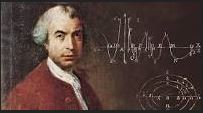
\includegraphics[height=.33\textheight,width=.33\textwidth]{boscovich.jpg}
\end{figure}
\begin{figure}
Karl F. Gauss
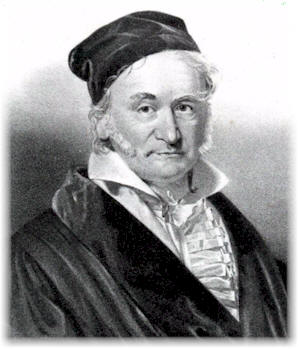
\includegraphics[height=.33\textheight,width=.33\textwidth]{gauss.jpg}
\end{figure}
\onslide<2->{\center --------------------------------------------------------------------}
\end{frame}
\begin{frame}
  \onslide<1->{\frametitle{Least Squares Luminaries} }
\begin{figure}
Peter Swerling
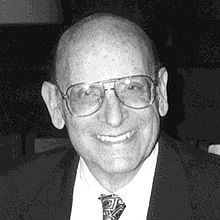
\includegraphics[height=.33\textheight,width=.33\textwidth]{Peter_Swerling.jpg}
\end{figure}
\begin{figure}
Rudolf Kalman
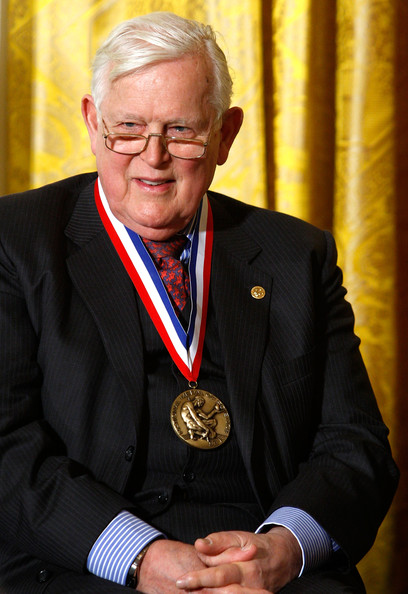
\includegraphics[height=.33\textheight,width=.33\textwidth]{RudolfKalman.jpg}
\end{figure}
\onslide<2->{\center --------------------------------------------------------------------}
\end{frame}

\begin{frame}
\onslide<1->{\frametitle{Kalman Filter Overview}
\framesubtitle{History}}
\begin{itemize}
\onslide<2->{\item Used in early 1960s by Schmidt on Apollo program}
\onslide<3->{\item  Kalman filters are now ubiquitous, especially in navigation}
  \begin{itemize}
     \onslide<4->{
       \item But also in signal processing, econometrics, finance, seismology, weather forecasting, sensor tracking
     }
  \end{itemize}
\end{itemize}
\onslide<5->{\center --------------------------------------------------------------------}
\end{frame}

\begin{frame}
\onslide<1->{\frametitle{Kalman Filter Overview}
\framesubtitle{KF uses in GPS}
}
\begin{itemize}
\onslide<2->{\item All three segments have Kalman filters}
\onslide<3->{\item CS:  ECEST = Ephemeris and Clock Estimator (legacy term), RTGx (JPL's Real-Time GPSY) and NRL's Ensemble Time Filter}
\onslide<4->{\item AEP's ECEST estimates inertial positions and velocities of SVs, solar pressure parameters, 
SV and MS clock error dynamics, and troposphere state at each MS}
\end{itemize}
\onslide<5->{\center --------------------------------------------------------------------}
\end{frame}

\begin{frame}
\onslide<1->{\frametitle{Kalman Filter Overview}
\framesubtitle{KF uses in GPS}
}
\begin{itemize}
\onslide<2->{\item In User Segment receivers, satellite nav software, and offline computations}
\onslide<3->{\item E.g., used in aircraft Operational Flight Programs (OFPs) and Inertial Navigation Systems (INSs) to integrate GPS and other external 
navaids to optimally estimate INS error states }
\onslide<4->{\item 1990s:  Paradigm shift in navigation:\\
  Was: "INS/GPS"\;\;\;\;  Is: "GPS/INS" }
\end{itemize}
\onslide<5->{\center --------------------------------------------------------------------}
\end{frame}


\begin{frame}
\onslide<1->{\frametitle{Kalman Filter Overview}}
\begin{itemize}
\onslide<2->{
	\item State estimation as branch of applied mathematics: 
	Kalman filtering uses techniques and results from many mathematical subjects:\\
linear algebra, differential equations, measure theory, probability, statistics, functional analysis (Hilbert space) 
}
\onslide<3->{
	\item But essentials are very intuitive
}	
	\begin{itemize}
	\onslide<4->{
		\item Can be understood with minimal math background (matrix algebra, calculus, probability and statistics )
	}
	\end{itemize}
\end{itemize}
\onslide<5->{\center --------------------------------------------------------------------}
\end{frame}

